\section{实验二：有效上下文窗口（子主张 S2）}\label{sec:s2}

本章用三把尺测量固定状态在损失上等效的上下文长度：位置衰减（\S\ref{sec:b1}）、
重复距离（\S\ref{sec:b2}）、等效滑窗（\S\ref{sec:b3}），外加精确检索的边界预实验（\S\ref{sec:b4}）。
截至本稿，前两把尺已完成（其中位置衰减以单流曲线替代），后两者未完成，如实标注。

\subsection{长文档位置衰减（B1）}\label{sec:b1}

\textbf{做成了什么。}完整的 B1（$5$--$10$ 篇 3 万--10 万字节文档的整篇曲线）尚未运行；
作为替代，本文已有两条\textbf{单流逐 patch 曲线}：96\,KB（seed 7）与 512\,KB（seed 11），
并在同一条流上做了重置频率扫描（E5）。

\textbf{结果（图 \ref{fig:e1} 右、图 \ref{fig:e5}）。}
96\,KB 流上逐 patch NLL 从前段 $0.4970$、中段 $0.6238$ 漂移到后段 $0.7784\nats$；
512\,KB 流同形状（$0.695\to0.874\nats$），全程无尖峰。
重置频率扫描（64\,KB 文本，状态每 $N$ token 重置回热启动快照，$N\in\{512,4096,16384,\infty\}$）
给出 $1.2147/1.0611/1.0430/1.0385\bits$——\textbf{单调下降、无 U 形}。

\begin{figure}[H]
\centering
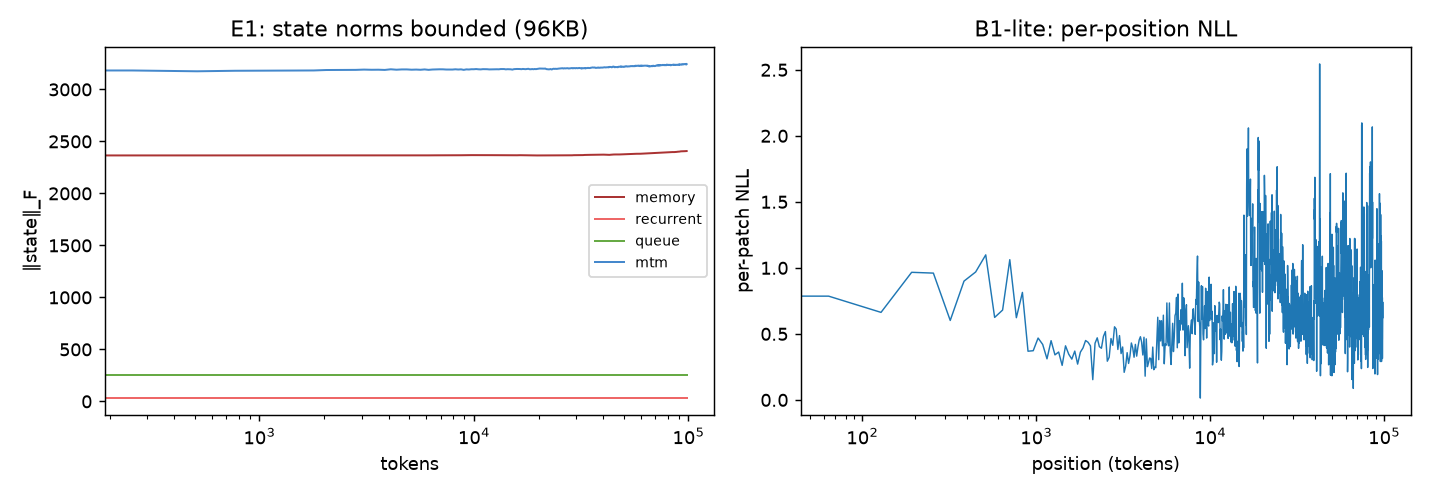
\includegraphics[width=\linewidth]{fig_e1_norms.png}
\caption{E1：96\,KB 单流的状态范数与逐 patch NLL。左：四分量范数（对数横轴）全程有界；
右：per-position 曲线（B1-lite），后段抬升与文本难度漂移一致（由 E5 判定，见正文）。}
\label{fig:e1}
\end{figure}

\begin{figure}[H]
\centering
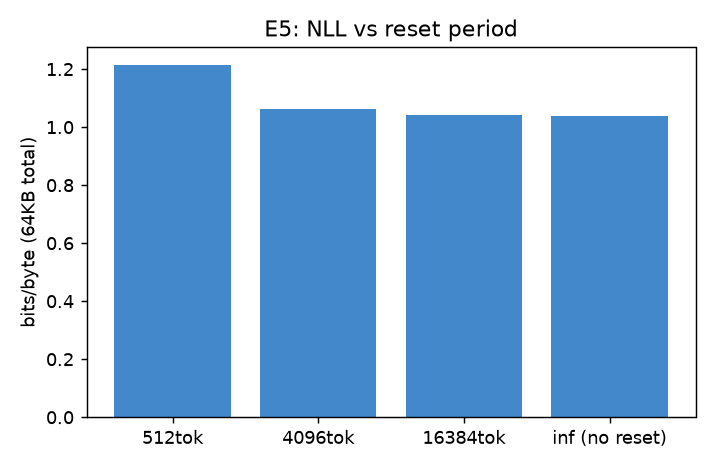
\includegraphics[width=0.62\linewidth]{fig_e5_reset.png}
\caption{E5：64\,KB 文本上，状态每 $N$ token 重置一次的总 bits/byte。
单调下降、无最优重置点 $\Rightarrow$ 在这个尺度上「永续写入」是纯收益、没有噪声累积。}
\label{fig:e5}
\end{figure}

\textbf{判定。}后段 NLL 的抬升\textbf{不是状态退化}：若存在噪声累积，重置频率扫描应出现 U 形
（重置太少则累积过噪声、太多则丢信息），而实测是单调的——每多写一点就多赚一点。
因此该抬升更保守的解释是流内文本难度/分布的漂移。这一点必须在论文里写清，
因为它决定了「永续写入」是否安全。\pending{B1 的整篇 vs 切段对照（真曲线）待补：
需要 5--10 篇长文档，实现见《论文大纲-B》第 3 章第 3.1 节。}

\subsection{自然重复的携带距离（B2）}\label{sec:b2}

\textbf{设计（免合成）。}在同一份 held-out 上流式取逐字节 NLL，扫描流内 $\mathrm{n}$-gram
（$n=8,16$）的第二次出现，按与第一次出现的距离分桶
（$<\!1$k / $1$k--$4$k / $4$k--$16$k / $16$k--$64$k / $>\!64$k 字节），
每个 gram 只计首次复现，指标为两次出现处 $\mathrm{n}$ 个字节 NLL 的均值（nats），
增益 $=$ 首次 $-$ 二次。

\textbf{结果（表 \ref{tab:b2}、图 \ref{fig:b2}）。}96\,KB 流、$n=8$：
增益\textbf{集中在 $<\!1$k 桶（$+0.0839\nats$，9384 对）}，
$1$k--$4$k 桶降至 $+0.019$，$4$k 以外为 $-0.013/-0.030/-0.015$；
$n=16$ 同形状（$<\!1$k 桶 $+0.0797$），但远桶样本数只有 $38/21$，噪声大。
512\,KB 流上 $<\!1$k 桶增益 $+0.0668\nats$（49716 对），
$1$k--$4$k 桶为 $-0.005$，$64$k--$256$k 与 $>\!256$k 桶分别在 $+0.006/-0.013$ 附近波动（图 \ref{fig:e1long} 右）。

% B2：自然重复距离分桶
\begin{table}[t]
\centering
\caption{B2 自然重复的复现距离分桶（96\,KB 流，$n=8$；已按修复后的分桶实现重跑）。
「距离」为与首次出现之间的字节距离（本模型中字节即 token）；
增益 $=$ 首次 $-$ 二次，正值表示第二次出现被更好地预测。
样本数互不相同这一点是分桶正确性的必要条件（见正文勘误说明）。
bucket 间比较并非完全受控——不同距离上重复的是不同的 $\mathrm{n}$-gram 群体，其首次出现难度本身不同。}
\label{tab:b2}
\small
\begin{tabular}{@{}lccccc@{}}
\toprule
距离桶 & $<\!1$k & $1$k--$4$k & $4$k--$16$k & $16$k--$64$k & $>\!64$k \\
\midrule
配对数量（$n=8$） & 9384 & 1225 & 1309 & 2708 & 382 \\
首次出现 NLL (nats) & $0.6863$ & $0.5167$ & $0.4773$ & $0.4665$ & $0.5082$ \\
二次出现 NLL (nats) & $0.6024$ & $0.4977$ & $0.4900$ & $0.4964$ & $0.5229$ \\
\midrule
\textbf{增益 (nats)} & $\mathbf{+0.0839}$ & $+0.0191$ & $-0.0127$ & $-0.0299$ & $-0.0148$ \\
\midrule
\multicolumn{6}{@{}l}{$n=16$（配对数量 3712 / 244 / 38 / 243 / 21）：增益 $+0.0797$ / $+0.0054$ / $-0.0467$ / $-0.0042$ / $+0.0021$} \\
\bottomrule
\end{tabular}
\end{table}


\begin{figure}[t]
\centering
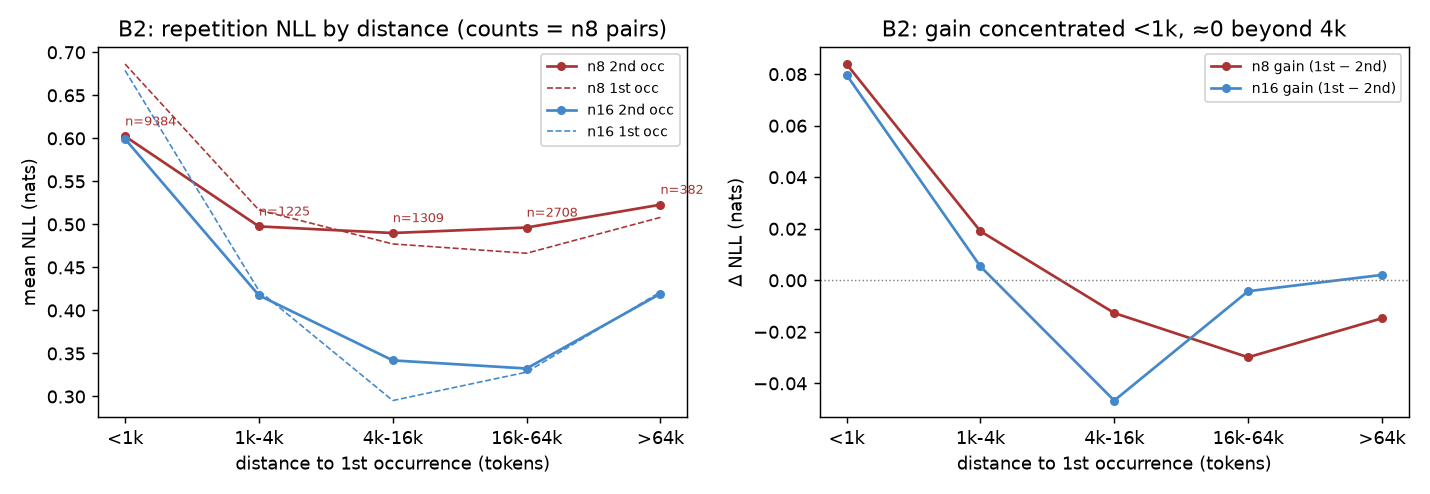
\includegraphics[width=\linewidth]{fig_b2_repetition.png}
\caption{B2：自然重复的复现 NLL 与距离（96\,KB 流）。
左：两桶的首次/二次出现 NLL（标注 $n=8$ 的配对数量）；
右：增益 $=$ 首次 $-$ 二次。增益集中在 $<\!1$k，$4$k 之外衰减到零甚至转负。}
\label{fig:b2}
\end{figure}

\textbf{组件归属（B2-freeze）。}把同一份 96\,KB 文本分别跑 5 个条件（全写、全程只读、冻结单分量），
$<\!1$k 桶增益为：write $+0.0839$、lock $-0.0050$、freeze \texttt{memory} $+0.0840$、
\textbf{freeze \texttt{recurrent} $-0.0043$}、freeze \texttt{queue}$+$\texttt{MTM} $+0.0837$
（表 \ref{tab:attr}(b)、图 \ref{fig:b2freeze}）。
\textbf{冻结 \texttt{recurrent} 精确抹平了复现增益}，代价层面也与全程只读等价
（bits/byte $2.153$ 对 $2.164$）。
这与 \S\ref{sec:s1-attr} 的 A6 结论自洽：该记忆存在 \texttt{recurrent} 里且是写入依赖的。

\begin{figure}[H]
\centering
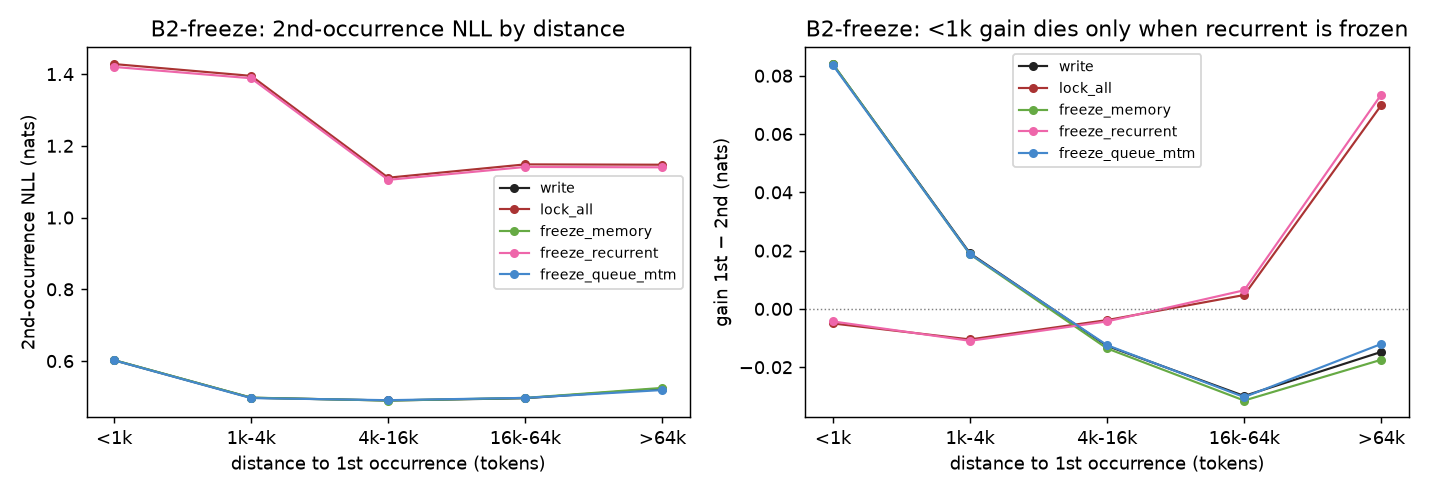
\includegraphics[width=\linewidth]{fig_b2_freeze.png}
\caption{B2-freeze：复现记忆的组件归属。左：二次出现的 NLL 曲线（5 个条件）；
右：增益 $=$ 首次 $-$ 二次。只有 \texttt{recurrent} 被冻结（或全程只读）时 $<\!1$k 增益消失，
冻结矩阵记忆与队列 $+$ MTM 无损。}
\label{fig:b2freeze}
\end{figure}

\textbf{一处必须公开的勘误。}早期版本曾得到「复现增益在 $<\!1$k 到 $>\!256$K 的所有距离桶内
零衰减」的结论，并据此写了「固定状态的记忆 $\ge256$K token 不衰减」。该结论\textbf{作废}：
分桶统计的实现把各桶的样本数写成了同一个值（每桶的数值被复制成同一份），
即「零衰减」是\textbf{所有桶都在报告同一个桶}造成的假象。
修复后重跑（96\,KB 与 512\,KB 两条流）即得到上表结果。
本文所有 B2 数字均为修复后数值；受影响的三张图已重画。
\textbf{教训}：分桶类统计必须在脚本里断言「各桶样本数互不相同且总和等于配对总数」，
否则一个变量作用域缺陷就会产出看起来干净、实则自证的曲线。

\begin{figure}[t]
\centering
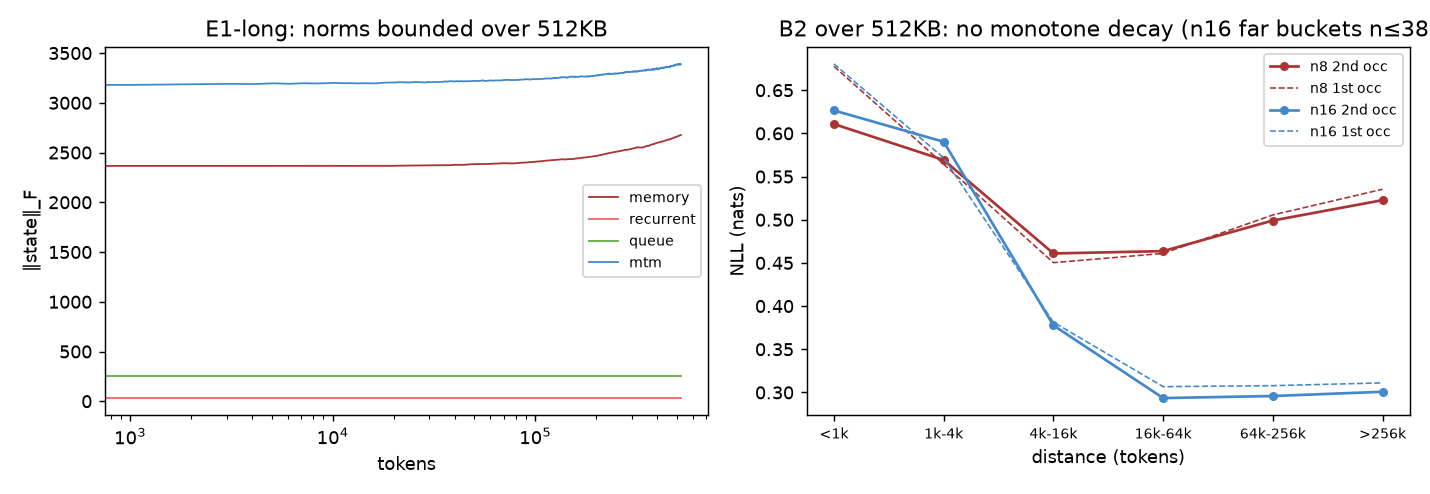
\includegraphics[width=\linewidth]{fig_e1long_b2.png}
\caption{E1-long：512\,KB 单流。左：状态范数（memory $\times1.13$、MTM $\times1.07$，STM/queue 恒定）；
右：B2 距离分桶的首次/二次出现 NLL——无单调衰减形状，$n=16$ 的远桶样本数 $\le1294$，读图需谨慎。}
\label{fig:e1long}
\end{figure}

\textbf{判定。}S2 的量化结论是：固定状态的\textbf{有效重复记忆距离约为 $1$--$4$k token}
（$<\!1$k 内增益显著，$4$k 外基本消失），且这一记忆\textbf{完全由 \texttt{recurrent} 承载}。
一个自洽的旁证：模型内部的通量结构里，队列的时标是 $64$ 槽 $\times$ $64$ token $=4096$ token
（表 \ref{tab:state}），与实测的 $1$--$4$k 量级吻合。\pending{该「时标吻合」是否有因果含义，
需要 C 线（受控注入 + 组件分离的遗忘曲线）才能判定，见附录 \ref{app:c1}。}

\subsection{等效滑窗基线（B3）}\label{sec:b3}

\textbf{设计（未完成）}：训一个 $2$--$4$ 层、局部因果窗口为 $W$ 的 byte Transformer 基线
（$W\in\{512,2\mathrm{k},8\mathrm{k},32\mathrm{k}\}$，数据同分布），
在 B1 的同一批长文档上跑同一套 teacher-forced 循环，得到各档 $W$ 的逐位置曲线，
对每个位置插值出与固定状态曲线最接近的 $W$，即「固定状态 $\approx W$ token 滑窗」的等效窗口。
来不及训练时的降级方案是引用公开滑窗基线并注明口径差异。
\pending{本项需要训练基线，超出「只用现成权重」的范围；这也是本文唯一能给出 S2 绝对数字的途径。}

\subsection{精确检索的边界（B4）}\label{sec:b4}

\textbf{设计（未完成）}：在距离 $d\in\{1\mathrm{k},4\mathrm{k},16\mathrm{k}\}$ 处插入 \texttt{key: value}，
文末 probe，统计精确匹配率。
\textbf{先行证据（指向「不擅长」）}：合成任务上的离散绑定测试（附录 \ref{app:g}）
显示该检查点对随机 ASCII 键值对的绑定很弱——
$k$ 次演示后答案位 NLL 仍在 $8.3$--$8.6$ bits（机会线 $8.23$），$k$ 增大不累积；
换成分布内的词对后曲线完全平（$5.0$--$5.2$ bits，与首字节机会线重合），
即这不是合成数据 OOD 造成的。据此本文\textbf{预判 needle 类精确检索不是本架构的强项}，
将其降级为限定 claim 与未来工作（\S\ref{sec:limits}），并如实报告而不是回避。

\subsection{小结：S2 部分成立}\label{sec:s2-summary}

\emph{S2 的部分结论}：有效窗口\textbf{显著大于 0}（$<\!1$k token 内复现增益 $+0.084\nats$、
且 $1$k--$4$k 仍有残余），但\textbf{远小于}早期误导性结论给出的 $\ge256$K：
固定状态在这个检查点上的自然重复记忆距离是 $1$--$4$k token。
因此「永续上下文」这一强主张\textbf{在当前证据下不成立}，
可辩护的表述是「固定大小状态等效于一段数 k token 的滑动记忆，且其容量不随历史增长而衰减」。
稳定性侧的正面证据（$512$\,KB 连续写入范数有界、重置频率扫描单调）说明\textbf{长度}不是问题，
瓶颈在\textbf{容量与写入/读出机制}——这正是下一步训练侧实验（F 线）要回答的问题（\S\ref{sec:discussion}）。
